\documentclass[10pt,pdf,hyperref={unicode}]{beamer}

\mode<presentation>
{
\usetheme{boxes}
\beamertemplatenavigationsymbolsempty

\setbeamertemplate{footline}[page number]
\setbeamersize{text margin left=0.5em, text margin right=0.5em}
}

\usepackage[utf8]{inputenc}
\usepackage[english, russian]{babel}
\usepackage{bm}
\usepackage{multirow}
\usepackage{ragged2e}
\usepackage{indentfirst}
\usepackage{multicol}
\usepackage{subfig}
\usepackage{amsmath,amssymb}
\usepackage{enumerate}
\usepackage{mathtools}
\usepackage{comment}
\usepackage{multicol}

\usepackage[all]{xy}

\usepackage{tikz}
\usetikzlibrary{positioning,arrows}

\tikzstyle{name} = [parameters]
\definecolor{name}{rgb}{0.5,0.5,0.5}

\usepackage{caption}
\captionsetup{skip=0pt,belowskip=0pt}

\newtheorem{rustheorem}{Теорема}
\newtheorem{russtatement}{Утверждение}
\newtheorem{rusdefinition}{Определение}

% colors
\definecolor{darkgreen}{rgb}{0.0, 0.2, 0.13}
\definecolor{darkcyan}{rgb}{0.0, 0.55, 0.55}

\AtBeginEnvironment{figure}{\setcounter{subfigure}{0}}

\captionsetup[subfloat]{labelformat=empty}

%----------------------------------------------------------------------------------------------------------

\title[]{Adversarial Schrödinger bridges}
\author{Ksenofontov\,G.\,S.\\[1ex] 
\small Isachenko\,R.\,V.}
\institute[]{Moscow Institute of Physics and Technology}
\date[2023]{\small 18\;may\;2024}

%---------------------------------------------------------------------------------------------------------
\begin{document}

\begin{frame}
\titlepage
\end{frame}

%---------------------------------------------------------------------------------------------------------- This implies that a learner has only a sample access to the (continuous) distributions and based on it has to recover the entire SB process (e.g., its drift) between the entire distributions.
\section{Research}
\begin{frame}{Research}
\bigskip
The high computational inference cost of diffusion-based Schrödinger Bridge approaches is investigated.
\begin{block}{Research objective~---}
suggest a method of solving Schrödinger Bridges without recovering entire Schrödinger Bridge process.
\end{block}
\begin{block}{Required to suggest}
\justifying
\begin{enumerate}[1.]
    \item algorithm of solving Schrödinger bridges problem that doesn't require recovering entire Schrödinger Bridge process,
    \item analysis of this algorithm.
\end{enumerate}
\end{block}
    \begin{block}{Solution}
        Use adversarial training instead of diffusion approaches.
    \end{block}
\end{frame}
% %---------------------------------------------------------------------------------------------------------
\section{Problem statement}
\begin{frame}{Problem statement}
It is given
\begin{enumerate}[1.]
    \item $\{x_i\}_{i=0}^N = X, \{y_j\}_{j=0}^N = Y$ -- two unpaired datasets,  where $x_i \sim \pi_0(x)$ and $y_j \sim \pi_1(y)$,
    \item $\mathbb{W}^{\gamma}$ -- path measure of reference Wiener process with drift $\sqrt{\gamma}$.
\end{enumerate}

Dynamic Schrödinger Bridge Problem finds the closest path measure $\mathbb{Q}$ with prescribed marginals of $\pi_0(x)$, $\pi_1(y)$ at times 0 and 1, to reference path measure $\mathbb{W}^{\gamma}$ in sense of KL-divergence, i.e.:

\begin{equation}
    \hat{\mathbb{Q}} = \arg\min_{\mathbb{Q}\in \mathcal{D}(\pi_0, \pi_1)} D_{KL}\mathbb{(Q||W}^\gamma),
    \label{eq:dyn}
\end{equation}
where $\mathcal{D}(\pi_0, \pi_1)$ is space of all path measures with prescribed marginals $\pi_0(x)$ and $\pi_1(y)$.
%  =  \mathcal{N}(x, \gamma\mathbb{I}) 

However, the solving of the problem requires to learn process that connects both marginals. It is computationally expensive, so, we propose a new approach that addresses this problem.

\end{frame}

% %----------------------------------------------------------------------------------------------------------
\section{Suggested Method}
\begin{frame}{Suggested Method}
~\\[-1mm]
Firstly, instead of solving dynamic version [\ref{eq:dyn}] of Schrödinger Bridge Problem we consider a Static formulation. With the same sets $X$ and $Y$ it is given joint distribution $p^{\mathbb{W}^\gamma}(x, y)$ of the reference Wiener process. Static Schrödinger Bridge Problem:

\begin{equation}
    \left\{ \begin{array}{c}
    q^*(x,y) = \arg\min_{q(x,y)} D_{KL}(q(x,y)||p^{\mathbb{W}^\gamma}(x,y)), \\
    \pi_0(x) = \int q(x,y)dy, \\
    \pi_1(y) = \int q(x,y)dx
    \end{array}\right.
    \label{eq:static}
\end{equation}

To solve (\ref{eq:static}) is used Iterational Proportional Fitting (IPF), which alternates between solving two half bridges (constrained only on one distribution). 
\end{frame}

\begin{frame}{Suggested Method}
~\\[-1mm]
To leverage adversarial approach we represent KL divergence in it's variational (dual) form (inspired by f-GAN [2]):
\begin{block}{Backward}
    \begin{equation*}
        \begin{split}
            \min_{p(x,y)\in\mathcal{D}(\cdot, \pi_1)} D_{KL}(p(x,y)||q^{i-1}(x,y)) = \min_{p(x,y)\in\mathcal{D}(\cdot, \pi_1)}\max_{D}\mathbb{E}_{(x,y)\sim p}\left[D(x,y)\right] - \\ - \mathbb{E}_{(x,y)\sim q^{i-1}}\left[e^{D(x,y) - 1}\right]
        \end{split}
    \end{equation*}
\end{block}

\begin{block}{Forward}
    \begin{equation*}
        \begin{split}
            \min_{q(x,y)\in\mathcal{D}(\pi_0, \cdot)} D_{KL}(q(x,y)||p^{i}(x,y)) = \min_{q(x,y)\in\mathcal{D}(\pi_0, \cdot)}\max_{D}\mathbb{E}_{(x,y)\sim q}\left[D(x,y)\right] - \\ - \mathbb{E}_{(x,y)\sim p^{i}}\left[e^{D(x,y) - 1}\right]
        \end{split}
    \end{equation*}
\end{block}
\end{frame}

\begin{frame}{Suggested Method}
~\\[-1mm]
In sense of converting one sample to another we want to learn conditional distribution:
\begin{block}{Backward}
    \begin{equation*}
        \begin{split}
             \min_{p(x,y)\in\mathcal{D}(\cdot, \pi_1)}\max_{D}\mathbb{E}_{(x,y)\sim p}\left[D(x,y)\right] - \mathbb{E}_{(x,y)\sim q^{i-1}}\left[e^{D(x,y) - 1}\right] = \\ = \min_{p(x|y)}\max_{D}\mathbb{E}_{y \sim \pi_1}\mathbb{E}_{x\sim p(x|y)}\left[D(x,y)\right] - \mathbb{E}_{x\sim\pi_0}\mathbb{E}_{y\sim q^{i-1}(y|x)}\left[e^{D(x,y) - 1}\right]
        \end{split}
    \end{equation*}
\end{block}

\begin{block}{Forward}
    \begin{equation*}
        \begin{split}
            \min_{q(x,y)\in\mathcal{D}(\pi_0, \cdot)}\max_{D}\mathbb{E}_{(x,y)\sim q}\left[D(x,y)\right] - \mathbb{E}_{(x,y)\sim p^{i}}\left[e^{D(x,y) - 1}\right] = \\ = \min_{q(y|x)}\max_{D}\mathbb{E}_{x\sim \pi_0}\mathbb{E}_{y\sim q(y|x)}\left[D(x,y)\right] - \mathbb{E}_{y\sim \pi_1}\mathbb{E}_{x\sim p^{i}(x|y)}\left[e^{D(x,y) - 1}\right]
        \end{split}
    \end{equation*}
\end{block}
\end{frame}

\begin{frame}{Suggested Method}
~\\[-1mm]
Using approach from Conditional GAN [3]:
\begin{block}{Backward}
    \begin{equation*}
        \begin{split}
             \min_{p(x|y)}\max_{D}\mathbb{E}_{y \sim \pi_1}\mathbb{E}_{x\sim p(x|y)}\left[D(x,y)\right] - \mathbb{E}_{x\sim\pi_0}\mathbb{E}_{y\sim q^{i-1}(y|x)}\left[e^{D(x,y) - 1}\right] = \\ = \min_{G}\max_{D}\mathbb{E}_{y \sim \pi_1}\mathbb{E}_{z\sim p(z)}\left[D(G(z|y),y)\right] - \mathbb{E}_{x\sim\pi_0}\mathbb{E}_{z\sim p(z)}\left[e^{D(x,F^{i-1}(z|x)) - 1}\right]
        \end{split}
    \end{equation*}
\end{block}

\begin{block}{Forward}
    \begin{equation*}
        \begin{split}
            \min_{q(y|x)}\max_{D}\mathbb{E}_{x\sim \pi_0}\mathbb{E}_{y\sim q(y|x)}\left[D(x,y)\right] - \mathbb{E}_{y\sim \pi_1}\mathbb{E}_{x\sim p^{i}(x|y)}\left[e^{D(x,y) - 1}\right] = \\ = \min_{F}\max_{D}\mathbb{E}_{x\sim \pi_0}\mathbb{E}_{z\sim p(z)}\left[D(x,F(z|x))\right] - \mathbb{E}_{y\sim \pi_1}\mathbb{E}_{z\sim p(z)}\left[e^{D(G^{i}(z|y),y) - 1}\right]
        \end{split}
    \end{equation*}
\end{block}
\end{frame}

\begin{frame}{Suggested Method}
~\\[-1mm]
    \begin{figure}
        \centering
        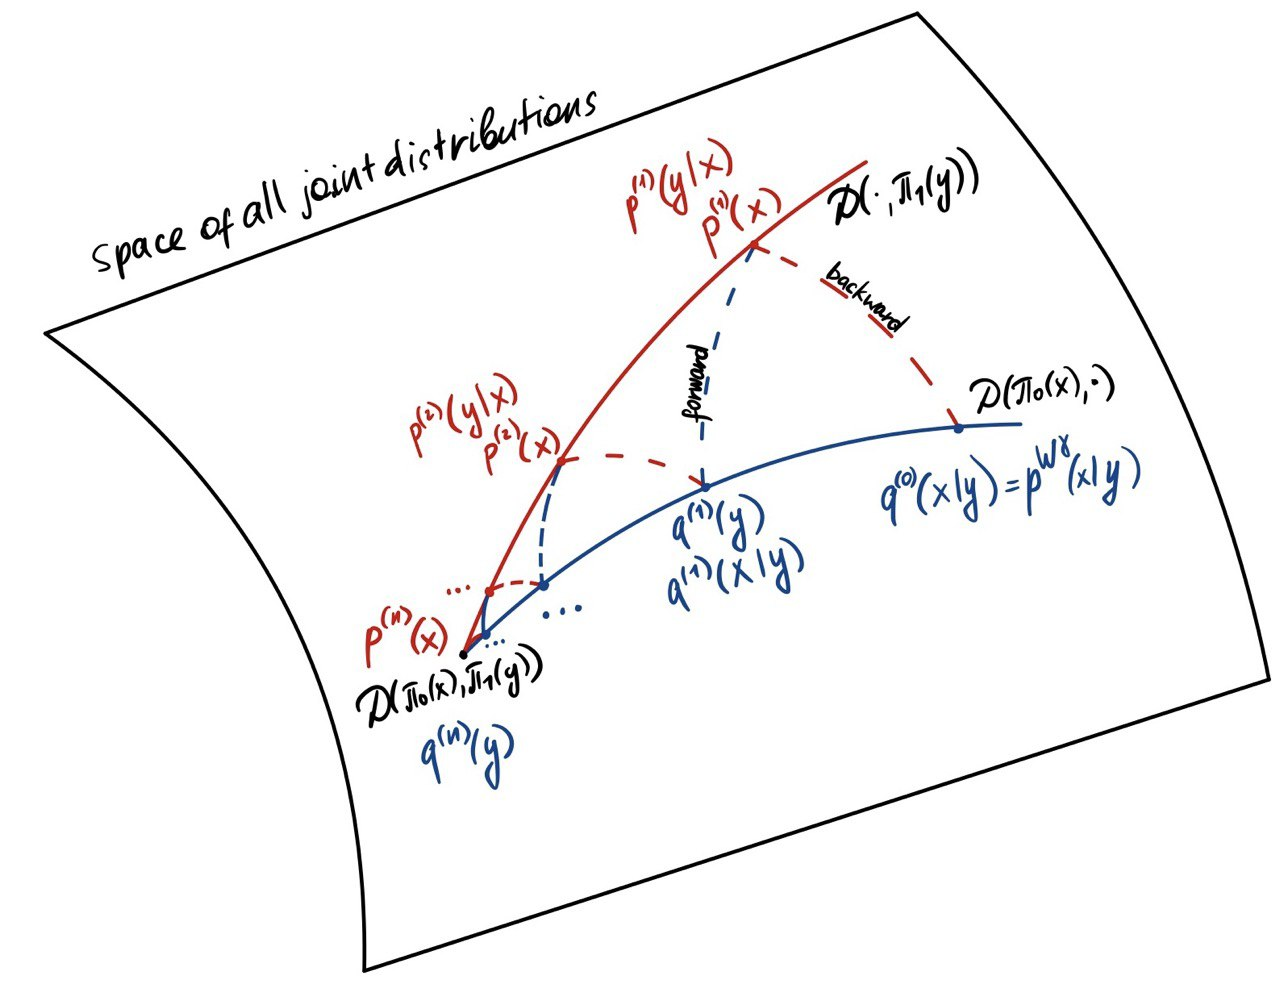
\includegraphics[width=0.8\linewidth]{slides/3d/figures/photo_2023-12-16_13-49-39.jpg}
    \end{figure}
\end{frame}

%----------------------------------------------------------------------------------------------------------
\section{Analysis of suggested method}
\begin{frame}{Analysis of suggested method}
\justifying

The graphs show the adversarial loss and final generative capabilities of adversarial bridges. 
\begin{figure}[h!]
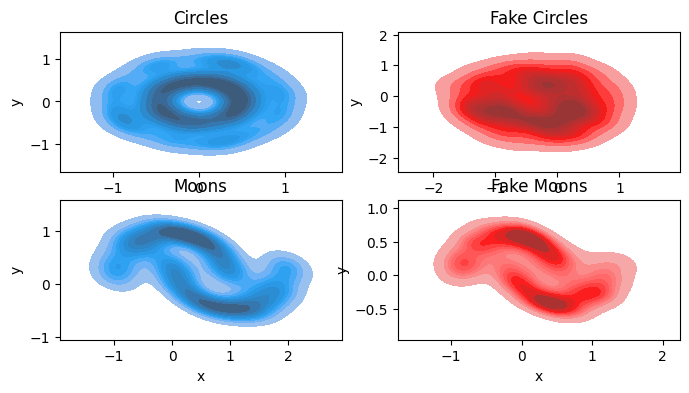
\includegraphics[width=0.45\textwidth]{figures/results.png}
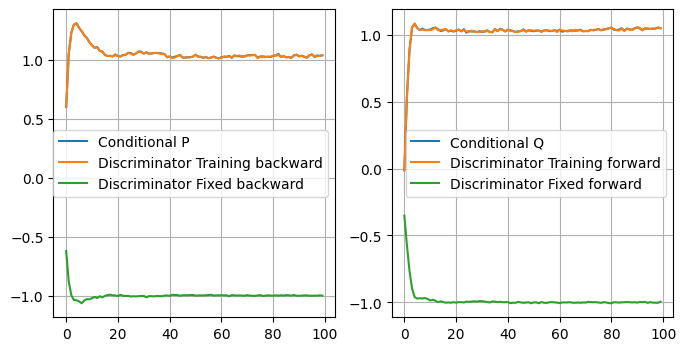
\includegraphics[width=0.45\textwidth]{figures/loss.png}
\end{figure}

It was conducted several experiments on data from multi-modal normal distributions, and no mode collapse problem was encountered.

\end{frame}

%----------------------------------------------------------------------------------------------------------
\section{Conclusion}
\begin{frame}{Conclusion}
\justifying
    \begin{enumerate}
        \justifying
        \item Proposed method of solving Schrodinger Bridge Problem with adversarial training.
        \item Conducted several experiments that shows great generative capability of proposed method, 
    \end{enumerate}
\end{frame}

%---------------------------------------------------------------------------------------------------------
\section{Related papers}
\begin{frame}{Related papers}
\begin{enumerate}[1.]
    \item Machine-learning approaches for the empirical Schrodinger bridge problem\footnote{\href{https://www.cl.cam.ac.uk/techreports/UCAM-CL-TR-958.pdf}{Machine-learning approaches for the empirical Schrodinger bridge problem, F. Vargas, 2021}}
    \item f-GAN: Training Generative Neural Samplers using Variational Divergence Minimization\footnote{\href{https://arxiv.org/abs/1606.00709}{f-GAN: Training Generative Neural Samplers using Variational Divergence Minimization, S. Nowozin, 2016}}
    \item Conditional Generative Adversarial Nets\footnote{\href{ https://arxiv.org/abs/1411.1784}{Conditional Generative Adversarial Nets, Mirza M. and Osindero S., 2014}}
\end{enumerate}
\end{frame}
%---------------------------------------------------------------------------------------------------------
\section{Future work plan}
\begin{frame}{Future work plan}
\begin{enumerate}[1.]
    \item Analyse numerical error and stability of proposed algorithm;
    \item Consider adversarial training without using IPF;
    \item Investigate generalization of $D_{KL}$ to other distances or metrics.
\end{enumerate}
\end{frame}
%----------------------------------------------------------------------------------------------------------

\end{document} 